\section{Transaction状态}
\begin{itemize}
    \item 活动态:初始状态;事务在执行期间保持此状态
    \item 部分提交:执行完最后一条语句后(此时要输出的结果数据可能还在内存buffer中)
    \item 失败:发现无法继续正常执行之后。
    \item 中止:事务回滚且数据库恢复到事务开始前的状态之后。中止后有两个选项:
       \begin{itemize}
          \item 重启事务:仅在无内部逻辑错误时方可执行。
          \item 终止事务。
       \end{itemize}
    \item 已提交:成功提交后。
\end{itemize}

\begin{figure}[H]
    \centering
    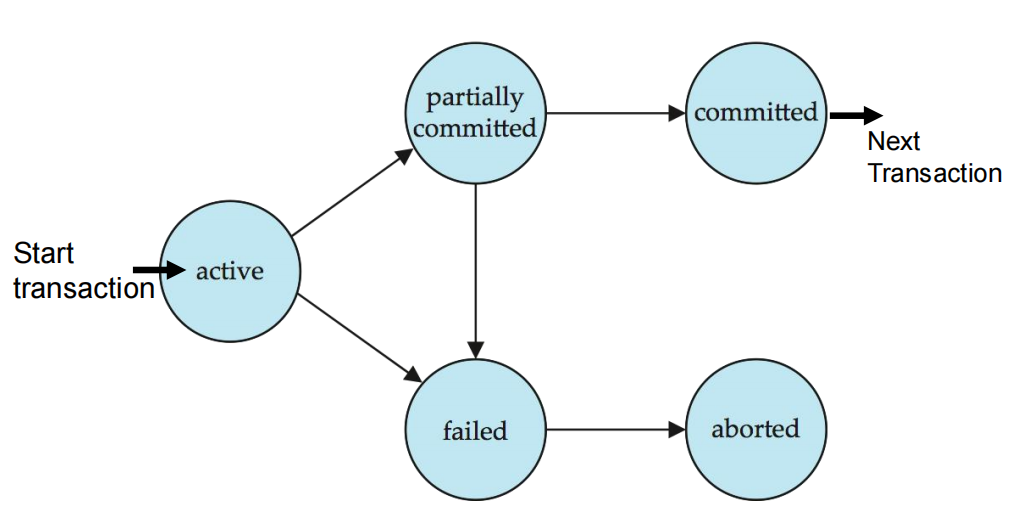
\includegraphics[width=0.8\linewidth]{image1.png}
    \caption{Transactions States}
    \label{}
\end{figure}